\documentclass[twoside]{book}

% Packages required by doxygen
\usepackage{calc}
\usepackage{doxygen}
\usepackage{graphicx}
\usepackage[utf8]{inputenc}
\usepackage{makeidx}
\usepackage{multicol}
\usepackage{multirow}
\usepackage{textcomp}
\usepackage[table]{xcolor}

% NLS support packages
\usepackage[T2A]{fontenc}
\usepackage[russian]{babel}

% Font selection
\usepackage[T1]{fontenc}
\usepackage{mathptmx}
\usepackage[scaled=.90]{helvet}
\usepackage{courier}
\usepackage{amssymb}
\usepackage{sectsty}
\renewcommand{\familydefault}{\sfdefault}
\allsectionsfont{%
  \fontseries{bc}\selectfont%
  \color{darkgray}%
}
\renewcommand{\DoxyLabelFont}{%
  \fontseries{bc}\selectfont%
  \color{darkgray}%
}

% Page & text layout
\usepackage{geometry}
\geometry{%
  a4paper,%
  top=2.5cm,%
  bottom=2.5cm,%
  left=2.5cm,%
  right=2.5cm%
}
\tolerance=750
\hfuzz=15pt
\hbadness=750
\setlength{\emergencystretch}{15pt}
\setlength{\parindent}{0cm}
\setlength{\parskip}{0.2cm}
\makeatletter
\renewcommand{\paragraph}{%
  \@startsection{paragraph}{4}{0ex}{-1.0ex}{1.0ex}{%
    \normalfont\normalsize\bfseries\SS@parafont%
  }%
}
\renewcommand{\subparagraph}{%
  \@startsection{subparagraph}{5}{0ex}{-1.0ex}{1.0ex}{%
    \normalfont\normalsize\bfseries\SS@subparafont%
  }%
}
\makeatother

% Headers & footers
\usepackage{fancyhdr}
\pagestyle{fancyplain}
\fancyhead[LE]{\fancyplain{}{\bfseries\thepage}}
\fancyhead[CE]{\fancyplain{}{}}
\fancyhead[RE]{\fancyplain{}{\bfseries\leftmark}}
\fancyhead[LO]{\fancyplain{}{\bfseries\rightmark}}
\fancyhead[CO]{\fancyplain{}{}}
\fancyhead[RO]{\fancyplain{}{\bfseries\thepage}}
\fancyfoot[LE]{\fancyplain{}{}}
\fancyfoot[CE]{\fancyplain{}{}}
\fancyfoot[RE]{\fancyplain{}{\bfseries\scriptsize Документация по Player\-\_\-\-Power. Последние изменения\-: Вс 10 Фев 2019 23\-:37\-:45. Создано системой Doxygen }}
\fancyfoot[LO]{\fancyplain{}{\bfseries\scriptsize Документация по Player\-\_\-\-Power. Последние изменения\-: Вс 10 Фев 2019 23\-:37\-:45. Создано системой Doxygen }}
\fancyfoot[CO]{\fancyplain{}{}}
\fancyfoot[RO]{\fancyplain{}{}}
\renewcommand{\footrulewidth}{0.4pt}
\renewcommand{\chaptermark}[1]{%
  \markboth{#1}{}%
}
\renewcommand{\sectionmark}[1]{%
  \markright{\thesection\ #1}%
}

% Indices & bibliography
\usepackage{natbib}
\usepackage[titles]{tocloft}
\setcounter{tocdepth}{3}
\setcounter{secnumdepth}{5}
\makeindex

% Custom commands
\newcommand{\clearemptydoublepage}{%
  \newpage{\pagestyle{empty}\cleardoublepage}%
}


%===== C O N T E N T S =====

\begin{document}

% Titlepage & ToC
\pagenumbering{roman}
\begin{titlepage}
\vspace*{7cm}
\begin{center}%
{\Large Player\-\_\-\-Power }\\
\vspace*{1cm}
{\large Создано системой Doxygen 1.8.6}\\
\vspace*{0.5cm}
{\small Вс 10 Фев 2019 23:37:45}\\
\end{center}
\end{titlepage}
\clearemptydoublepage
\tableofcontents
\clearemptydoublepage
\pagenumbering{arabic}

%--- Begin generated contents ---
\chapter{Алфавитный указатель пространств имен}
\section{Пакеты}
Полный список документированных пакетов.\begin{DoxyCompactList}
\item\contentsline{section}{{\bf Player\-\_\-\-Power} }{\pageref{namespace_player___power}}{}
\end{DoxyCompactList}

\chapter{Иерархический список классов}
\section{Иерархия классов}
Иерархия классов.\begin{DoxyCompactList}
\item \contentsline{section}{Player\-\_\-\-Power.\-I\-Player}{\pageref{interface_player___power_1_1_i_player}}{}
\begin{DoxyCompactList}
\item \contentsline{section}{Player\-\_\-\-Power.\-Player}{\pageref{class_player___power_1_1_player}}{}
\item \contentsline{section}{Player\-\_\-\-Power.\-Power}{\pageref{class_player___power_1_1_power}}{}
\begin{DoxyCompactList}
\item \contentsline{section}{Player\-\_\-\-Power.\-Panasonic}{\pageref{class_player___power_1_1_panasonic}}{}
\item \contentsline{section}{Player\-\_\-\-Power.\-Samsung}{\pageref{class_player___power_1_1_samsung}}{}
\item \contentsline{section}{Player\-\_\-\-Power.\-Sony}{\pageref{class_player___power_1_1_sony}}{}
\end{DoxyCompactList}
\end{DoxyCompactList}
\item \contentsline{section}{Player\-\_\-\-Power.\-I\-Voltage}{\pageref{interface_player___power_1_1_i_voltage}}{}
\item Ninject\-Module\begin{DoxyCompactList}
\item \contentsline{section}{Player\-\_\-\-Power.\-My\-Config\-Module\-\_\-\-V110}{\pageref{class_player___power_1_1_my_config_module___v110}}{}
\item \contentsline{section}{Player\-\_\-\-Power.\-My\-Config\-Module\-\_\-\-V127}{\pageref{class_player___power_1_1_my_config_module___v127}}{}
\item \contentsline{section}{Player\-\_\-\-Power.\-My\-Config\-Module\-\_\-\-V220}{\pageref{class_player___power_1_1_my_config_module___v220}}{}
\item \contentsline{section}{Player\-\_\-\-Power.\-My\-Config\-Module\-\_\-\-V380}{\pageref{class_player___power_1_1_my_config_module___v380}}{}
\end{DoxyCompactList}
\end{DoxyCompactList}

\chapter{Алфавитный указатель классов}
\section{Классы}
Классы с их кратким описанием.\begin{DoxyCompactList}
\item\contentsline{section}{{\bf Player\-\_\-\-Power.\-I\-Player} }{\pageref{interface_player___power_1_1_i_player}}{}
\item\contentsline{section}{{\bf Player\-\_\-\-Power.\-I\-Voltage} }{\pageref{interface_player___power_1_1_i_voltage}}{}
\item\contentsline{section}{{\bf Player\-\_\-\-Power.\-My\-Config\-Module\-\_\-\-V110} }{\pageref{class_player___power_1_1_my_config_module___v110}}{}
\item\contentsline{section}{{\bf Player\-\_\-\-Power.\-My\-Config\-Module\-\_\-\-V127} }{\pageref{class_player___power_1_1_my_config_module___v127}}{}
\item\contentsline{section}{{\bf Player\-\_\-\-Power.\-My\-Config\-Module\-\_\-\-V220} }{\pageref{class_player___power_1_1_my_config_module___v220}}{}
\item\contentsline{section}{{\bf Player\-\_\-\-Power.\-My\-Config\-Module\-\_\-\-V380} }{\pageref{class_player___power_1_1_my_config_module___v380}}{}
\item\contentsline{section}{{\bf Player\-\_\-\-Power.\-Panasonic} }{\pageref{class_player___power_1_1_panasonic}}{}
\item\contentsline{section}{{\bf Player\-\_\-\-Power.\-Player} }{\pageref{class_player___power_1_1_player}}{}
\item\contentsline{section}{{\bf Player\-\_\-\-Power.\-Power} }{\pageref{class_player___power_1_1_power}}{}
\item\contentsline{section}{{\bf Player\-\_\-\-Power.\-Samsung} }{\pageref{class_player___power_1_1_samsung}}{}
\item\contentsline{section}{{\bf Player\-\_\-\-Power.\-Sony} }{\pageref{class_player___power_1_1_sony}}{}
\end{DoxyCompactList}

\chapter{Пространства имен}
\section{Пакет Player\-\_\-\-Power}
\label{namespace_player___power}\index{Player\-\_\-\-Power@{Player\-\_\-\-Power}}
\subsection*{Классы}
\begin{DoxyCompactItemize}
\item 
class {\bf Power}
\item 
interface {\bf I\-Voltage}
\item 
class {\bfseries Voltage\-V110}
\item 
class {\bfseries Voltage\-V127}
\item 
class {\bfseries Voltage\-V220}
\item 
class {\bfseries Voltage\-V380}
\item 
interface {\bf I\-Player}
\item 
class {\bf Samsung}
\item 
class {\bf Panasonic}
\item 
class {\bf Sony}
\item 
class {\bf Player}
\item 
class {\bf My\-Config\-Module\-\_\-\-V110}
\item 
class {\bf My\-Config\-Module\-\_\-\-V127}
\item 
class {\bf My\-Config\-Module\-\_\-\-V220}
\item 
class {\bf My\-Config\-Module\-\_\-\-V380}
\item 
class {\bfseries Program}
\end{DoxyCompactItemize}

\chapter{Классы}
\section{Интерфейс Player\-\_\-\-Power.\-I\-Player}
\label{interface_player___power_1_1_i_player}\index{Player\-\_\-\-Power.\-I\-Player@{Player\-\_\-\-Power.\-I\-Player}}


Граф наследования\-:Player\-\_\-\-Power.\-I\-Player\-:
\nopagebreak
\begin{figure}[H]
\begin{center}
\leavevmode
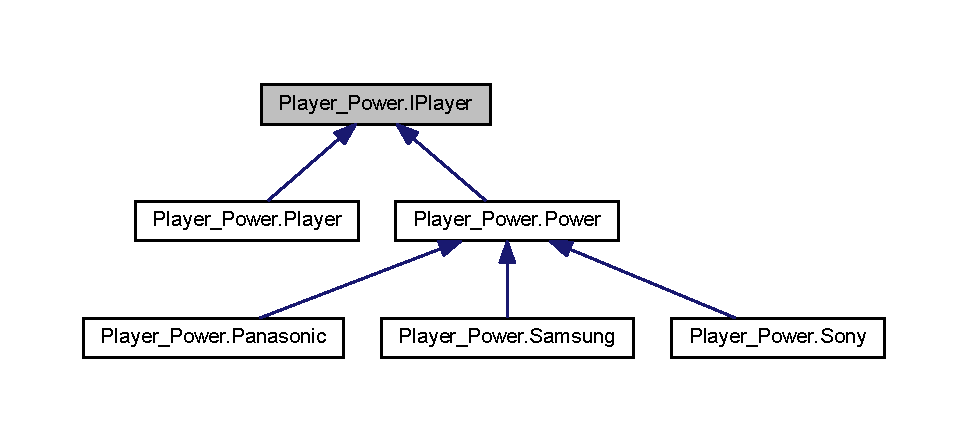
\includegraphics[width=350pt]{interface_player___power_1_1_i_player__inherit__graph}
\end{center}
\end{figure}
\subsection*{Открытые члены}
\begin{DoxyCompactItemize}
\item 
void {\bfseries Pause} ()\label{interface_player___power_1_1_i_player_a80b3a2311cf29cb5d11715246d33fc05}

\item 
void {\bfseries Start} ()\label{interface_player___power_1_1_i_player_a7836ccd9e36c42524aee2e3392823cb0}

\item 
void {\bfseries Stop} ()\label{interface_player___power_1_1_i_player_ab1020806df8f4b7d0f4c58a2c2f6e037}

\end{DoxyCompactItemize}


Объявления и описания членов интерфейса находятся в файле\-:\begin{DoxyCompactItemize}
\item 
Program.\-cs\end{DoxyCompactItemize}

\section{Интерфейс Player\-\_\-\-Power.\-I\-Voltage}
\label{interface_player___power_1_1_i_voltage}\index{Player\-\_\-\-Power.\-I\-Voltage@{Player\-\_\-\-Power.\-I\-Voltage}}


Граф наследования\-:Player\-\_\-\-Power.\-I\-Voltage\-:
\nopagebreak
\begin{figure}[H]
\begin{center}
\leavevmode
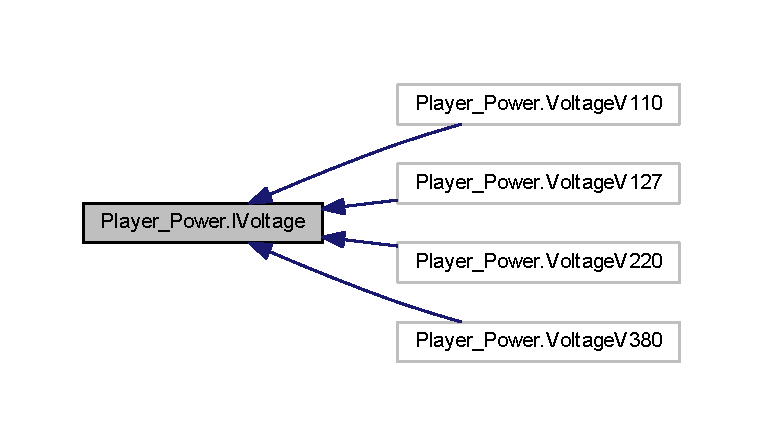
\includegraphics[width=350pt]{interface_player___power_1_1_i_voltage__inherit__graph}
\end{center}
\end{figure}
\subsection*{Открытые члены}
\begin{DoxyCompactItemize}
\item 
int {\bfseries Get\-Voltage} ()\label{interface_player___power_1_1_i_voltage_a3be8758f9d6d9ae3ce0d8344bcc39ee1}

\end{DoxyCompactItemize}


Объявления и описания членов интерфейса находятся в файле\-:\begin{DoxyCompactItemize}
\item 
Program.\-cs\end{DoxyCompactItemize}

\section{Класс Player\-\_\-\-Power.\-My\-Config\-Module\-\_\-\-V110}
\label{class_player___power_1_1_my_config_module___v110}\index{Player\-\_\-\-Power.\-My\-Config\-Module\-\_\-\-V110@{Player\-\_\-\-Power.\-My\-Config\-Module\-\_\-\-V110}}


Граф наследования\-:Player\-\_\-\-Power.\-My\-Config\-Module\-\_\-\-V110\-:
\nopagebreak
\begin{figure}[H]
\begin{center}
\leavevmode
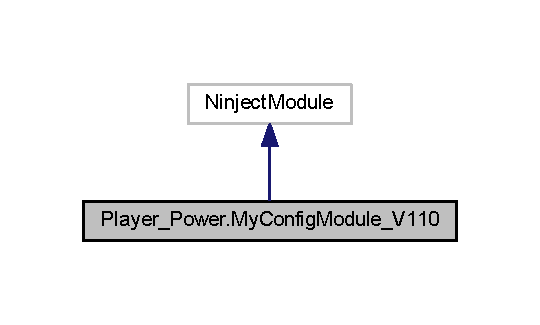
\includegraphics[width=259pt]{class_player___power_1_1_my_config_module___v110__inherit__graph}
\end{center}
\end{figure}


Граф связей класса Player\-\_\-\-Power.\-My\-Config\-Module\-\_\-\-V110\-:
\nopagebreak
\begin{figure}[H]
\begin{center}
\leavevmode
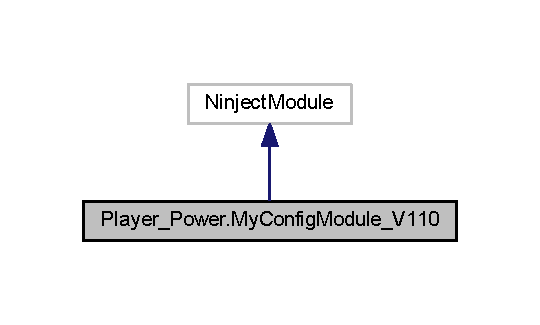
\includegraphics[width=259pt]{class_player___power_1_1_my_config_module___v110__coll__graph}
\end{center}
\end{figure}
\subsection*{Открытые члены}
\begin{DoxyCompactItemize}
\item 
override void {\bfseries Load} ()\label{class_player___power_1_1_my_config_module___v110_a9fb768c54955b78c1bdeb8d4d79b071a}

\end{DoxyCompactItemize}


Объявления и описания членов класса находятся в файле\-:\begin{DoxyCompactItemize}
\item 
Program.\-cs\end{DoxyCompactItemize}

\section{Класс Player\-\_\-\-Power.\-My\-Config\-Module\-\_\-\-V127}
\label{class_player___power_1_1_my_config_module___v127}\index{Player\-\_\-\-Power.\-My\-Config\-Module\-\_\-\-V127@{Player\-\_\-\-Power.\-My\-Config\-Module\-\_\-\-V127}}


Граф наследования\-:Player\-\_\-\-Power.\-My\-Config\-Module\-\_\-\-V127\-:
\nopagebreak
\begin{figure}[H]
\begin{center}
\leavevmode
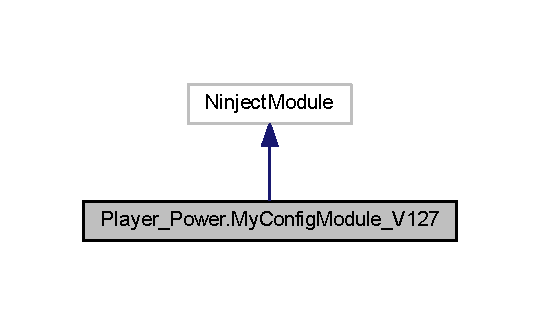
\includegraphics[width=259pt]{class_player___power_1_1_my_config_module___v127__inherit__graph}
\end{center}
\end{figure}


Граф связей класса Player\-\_\-\-Power.\-My\-Config\-Module\-\_\-\-V127\-:
\nopagebreak
\begin{figure}[H]
\begin{center}
\leavevmode
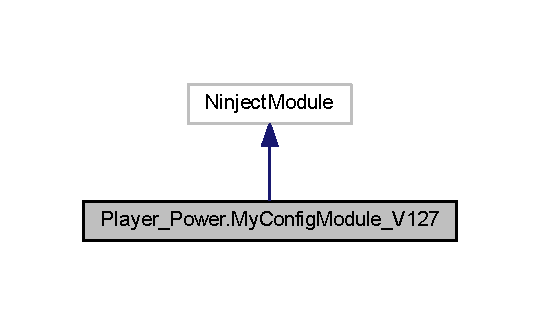
\includegraphics[width=259pt]{class_player___power_1_1_my_config_module___v127__coll__graph}
\end{center}
\end{figure}
\subsection*{Открытые члены}
\begin{DoxyCompactItemize}
\item 
override void {\bfseries Load} ()\label{class_player___power_1_1_my_config_module___v127_a9cbed41a11edf4706a45f381ef91b7ee}

\end{DoxyCompactItemize}


Объявления и описания членов класса находятся в файле\-:\begin{DoxyCompactItemize}
\item 
Program.\-cs\end{DoxyCompactItemize}

\section{Класс Player\-\_\-\-Power.\-My\-Config\-Module\-\_\-\-V220}
\label{class_player___power_1_1_my_config_module___v220}\index{Player\-\_\-\-Power.\-My\-Config\-Module\-\_\-\-V220@{Player\-\_\-\-Power.\-My\-Config\-Module\-\_\-\-V220}}


Граф наследования\-:Player\-\_\-\-Power.\-My\-Config\-Module\-\_\-\-V220\-:
\nopagebreak
\begin{figure}[H]
\begin{center}
\leavevmode
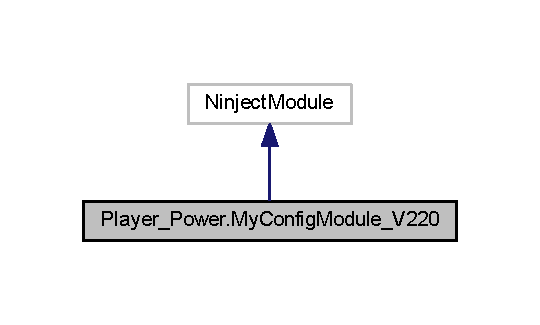
\includegraphics[width=259pt]{class_player___power_1_1_my_config_module___v220__inherit__graph}
\end{center}
\end{figure}


Граф связей класса Player\-\_\-\-Power.\-My\-Config\-Module\-\_\-\-V220\-:
\nopagebreak
\begin{figure}[H]
\begin{center}
\leavevmode
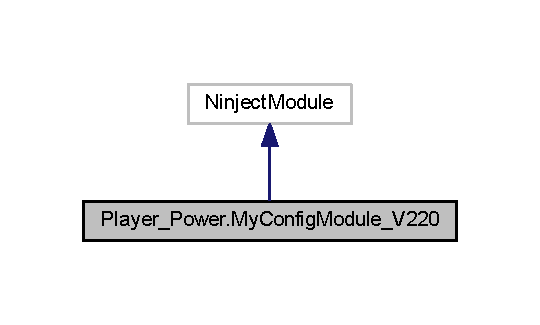
\includegraphics[width=259pt]{class_player___power_1_1_my_config_module___v220__coll__graph}
\end{center}
\end{figure}
\subsection*{Открытые члены}
\begin{DoxyCompactItemize}
\item 
override void {\bfseries Load} ()\label{class_player___power_1_1_my_config_module___v220_aac02cf2b257498e7786c0ff13c39b64e}

\end{DoxyCompactItemize}


Объявления и описания членов класса находятся в файле\-:\begin{DoxyCompactItemize}
\item 
Program.\-cs\end{DoxyCompactItemize}

\section{Класс Player\-\_\-\-Power.\-My\-Config\-Module\-\_\-\-V380}
\label{class_player___power_1_1_my_config_module___v380}\index{Player\-\_\-\-Power.\-My\-Config\-Module\-\_\-\-V380@{Player\-\_\-\-Power.\-My\-Config\-Module\-\_\-\-V380}}


Граф наследования\-:Player\-\_\-\-Power.\-My\-Config\-Module\-\_\-\-V380\-:
\nopagebreak
\begin{figure}[H]
\begin{center}
\leavevmode
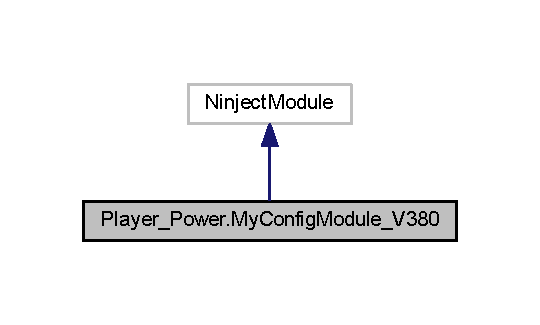
\includegraphics[width=259pt]{class_player___power_1_1_my_config_module___v380__inherit__graph}
\end{center}
\end{figure}


Граф связей класса Player\-\_\-\-Power.\-My\-Config\-Module\-\_\-\-V380\-:
\nopagebreak
\begin{figure}[H]
\begin{center}
\leavevmode
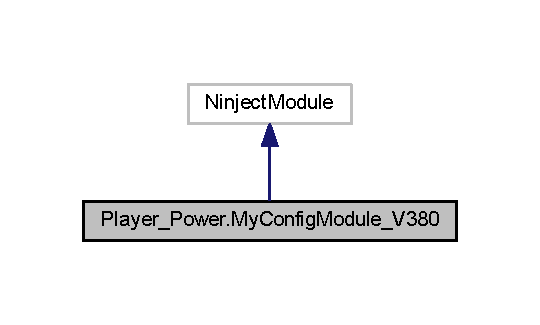
\includegraphics[width=259pt]{class_player___power_1_1_my_config_module___v380__coll__graph}
\end{center}
\end{figure}
\subsection*{Открытые члены}
\begin{DoxyCompactItemize}
\item 
override void {\bfseries Load} ()\label{class_player___power_1_1_my_config_module___v380_a09fe5e47f6d3b8cb32fa687e609296e6}

\end{DoxyCompactItemize}


Объявления и описания членов класса находятся в файле\-:\begin{DoxyCompactItemize}
\item 
Program.\-cs\end{DoxyCompactItemize}

\section{Класс Player\-\_\-\-Power.\-Panasonic}
\label{class_player___power_1_1_panasonic}\index{Player\-\_\-\-Power.\-Panasonic@{Player\-\_\-\-Power.\-Panasonic}}


Граф наследования\-:Player\-\_\-\-Power.\-Panasonic\-:
\nopagebreak
\begin{figure}[H]
\begin{center}
\leavevmode
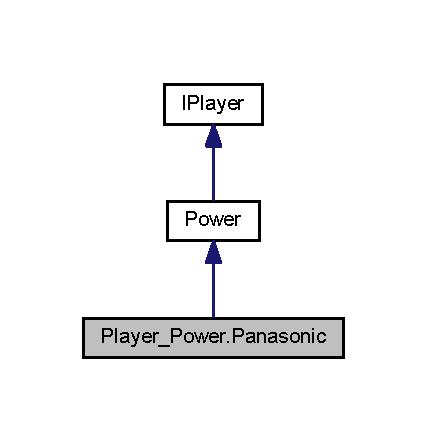
\includegraphics[width=205pt]{class_player___power_1_1_panasonic__inherit__graph}
\end{center}
\end{figure}


Граф связей класса Player\-\_\-\-Power.\-Panasonic\-:
\nopagebreak
\begin{figure}[H]
\begin{center}
\leavevmode
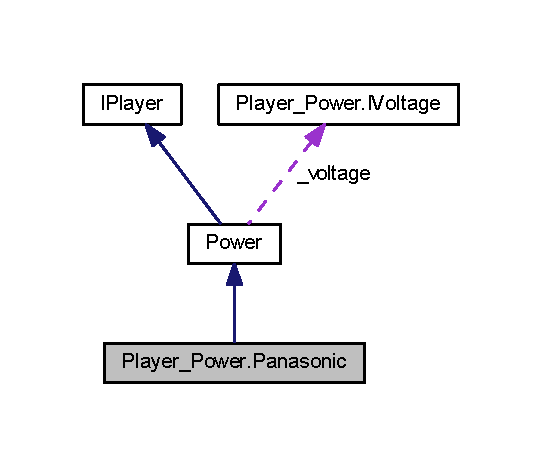
\includegraphics[width=260pt]{class_player___power_1_1_panasonic__coll__graph}
\end{center}
\end{figure}
\subsection*{Открытые члены}
\begin{DoxyCompactItemize}
\item 
{\bf Panasonic}({\bf I\-Player} player, \\*
{\bf I\-Voltage} voltage) override \\*
void {\bfseries Pause} ()\label{class_player___power_1_1_panasonic_ae3f5b9c9af4e25fe6364b94e2fde4d18}

\item 
override void {\bfseries Start} ()\label{class_player___power_1_1_panasonic_a78e006c41c0861f69dcbd66a99213023}

\item 
override void {\bfseries Stop} ()\label{class_player___power_1_1_panasonic_ac14217ffc5201092eccf0f62db67b9f0}

\item 
override void {\bfseries Show\-Voltage} ()\label{class_player___power_1_1_panasonic_ae854054c72fb47d085280d96d89feb63}

\end{DoxyCompactItemize}
\subsection*{Дополнительные унаследованные члены}


Объявления и описания членов класса находятся в файле\-:\begin{DoxyCompactItemize}
\item 
Program.\-cs\end{DoxyCompactItemize}

\section{Класс Player\-\_\-\-Power.\-Player}
\label{class_player___power_1_1_player}\index{Player\-\_\-\-Power.\-Player@{Player\-\_\-\-Power.\-Player}}


Граф наследования\-:Player\-\_\-\-Power.\-Player\-:
\nopagebreak
\begin{figure}[H]
\begin{center}
\leavevmode
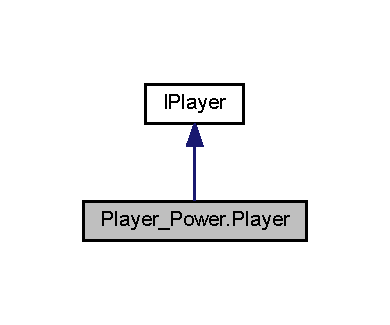
\includegraphics[width=187pt]{class_player___power_1_1_player__inherit__graph}
\end{center}
\end{figure}


Граф связей класса Player\-\_\-\-Power.\-Player\-:
\nopagebreak
\begin{figure}[H]
\begin{center}
\leavevmode
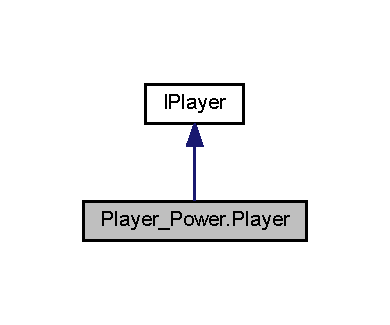
\includegraphics[width=187pt]{class_player___power_1_1_player__coll__graph}
\end{center}
\end{figure}
\subsection*{Открытые члены}
\begin{DoxyCompactItemize}
\item 
void {\bfseries Pause} ()\label{class_player___power_1_1_player_a5536f99c27bd3e8b3c14bad2ac3db63b}

\item 
void {\bfseries Start} ()\label{class_player___power_1_1_player_a2cce62aa8b76d5ea7a097b3d7e6c42a0}

\item 
void {\bfseries Stop} ()\label{class_player___power_1_1_player_aba865811451a1a1d2202c455331cc8aa}

\end{DoxyCompactItemize}


Объявления и описания членов класса находятся в файле\-:\begin{DoxyCompactItemize}
\item 
Program.\-cs\end{DoxyCompactItemize}

\section{Класс Player\-\_\-\-Power.\-Power}
\label{class_player___power_1_1_power}\index{Player\-\_\-\-Power.\-Power@{Player\-\_\-\-Power.\-Power}}


Граф наследования\-:Player\-\_\-\-Power.\-Power\-:
\nopagebreak
\begin{figure}[H]
\begin{center}
\leavevmode
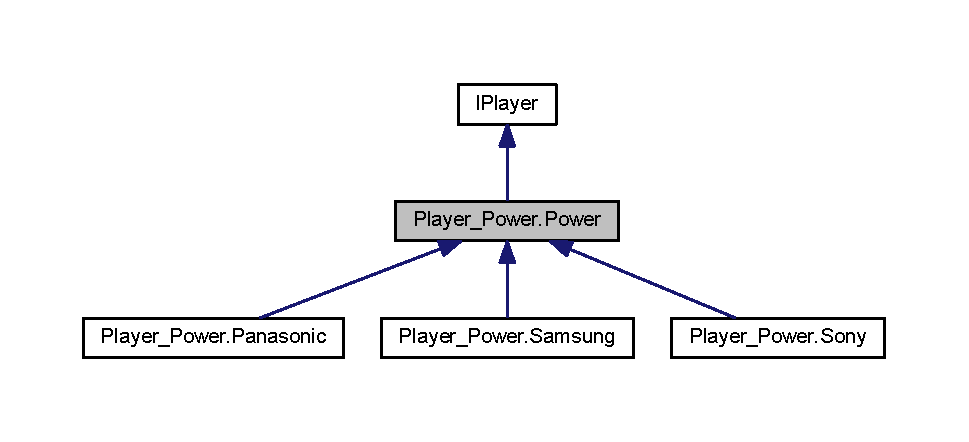
\includegraphics[width=350pt]{class_player___power_1_1_power__inherit__graph}
\end{center}
\end{figure}


Граф связей класса Player\-\_\-\-Power.\-Power\-:
\nopagebreak
\begin{figure}[H]
\begin{center}
\leavevmode
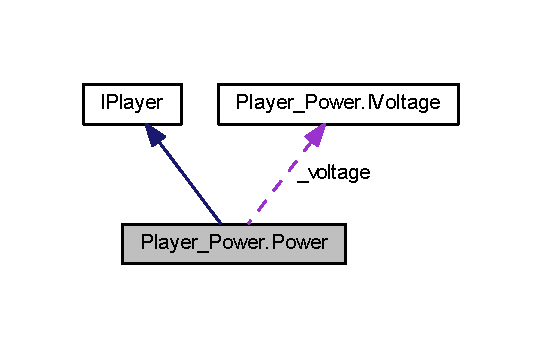
\includegraphics[width=260pt]{class_player___power_1_1_power__coll__graph}
\end{center}
\end{figure}
\subsection*{Открытые члены}
\begin{DoxyCompactItemize}
\item 
abstract void {\bfseries Pause} ()\label{class_player___power_1_1_power_a3c130b04215027dde6380b8cc43b8331}

\item 
abstract void {\bfseries Start} ()\label{class_player___power_1_1_power_a136fcc3925c43b987ba5ecc13fee498b}

\item 
abstract void {\bfseries Stop} ()\label{class_player___power_1_1_power_a0df6e9fbbad3f2647257568d6d190e4c}

\item 
virtual void {\bfseries Show\-Voltage} ()\label{class_player___power_1_1_power_a7c930922908710572baf5a04122b4a09}

\end{DoxyCompactItemize}
\subsection*{Свойства}
\begin{DoxyCompactItemize}
\item 
int {\bfseries Voltage}\hspace{0.3cm}{\ttfamily  [get, set]}\label{class_player___power_1_1_power_a6f18f8e34d5b60ec23513b790899b0c3}

\end{DoxyCompactItemize}


Объявления и описания членов класса находятся в файле\-:\begin{DoxyCompactItemize}
\item 
Program.\-cs\end{DoxyCompactItemize}

\section{Класс Player\-\_\-\-Power.\-Samsung}
\label{class_player___power_1_1_samsung}\index{Player\-\_\-\-Power.\-Samsung@{Player\-\_\-\-Power.\-Samsung}}


Граф наследования\-:Player\-\_\-\-Power.\-Samsung\-:
\nopagebreak
\begin{figure}[H]
\begin{center}
\leavevmode
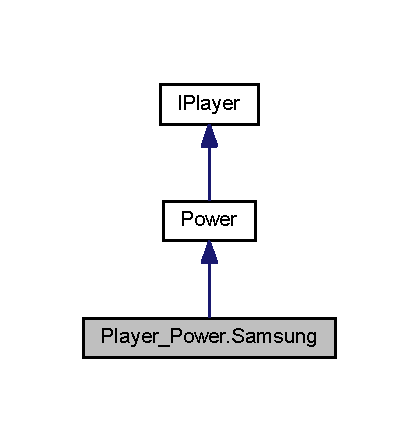
\includegraphics[width=201pt]{class_player___power_1_1_samsung__inherit__graph}
\end{center}
\end{figure}


Граф связей класса Player\-\_\-\-Power.\-Samsung\-:
\nopagebreak
\begin{figure}[H]
\begin{center}
\leavevmode
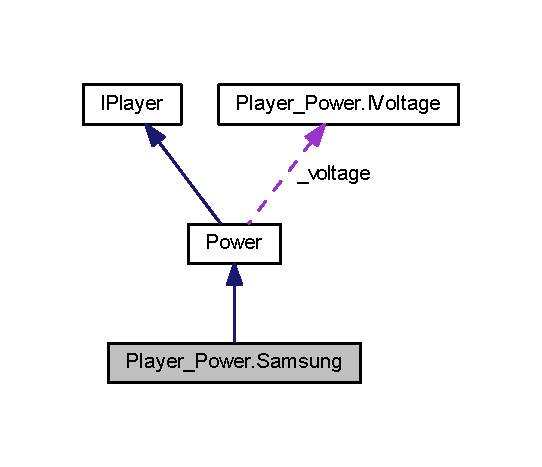
\includegraphics[width=260pt]{class_player___power_1_1_samsung__coll__graph}
\end{center}
\end{figure}
\subsection*{Открытые члены}
\begin{DoxyCompactItemize}
\item 
{\bf Samsung}({\bf I\-Player} player, \\*
{\bf I\-Voltage} voltage) override \\*
void {\bfseries Pause} ()\label{class_player___power_1_1_samsung_aedd1ed961f6aeba8a9a30c46af4a12f6}

\item 
override void {\bfseries Start} ()\label{class_player___power_1_1_samsung_ae9dc71245f1f468e69dd61adf45f1368}

\item 
override void {\bfseries Stop} ()\label{class_player___power_1_1_samsung_a5f17f99559769aeaff7c78dcf6b29efc}

\end{DoxyCompactItemize}
\subsection*{Дополнительные унаследованные члены}


Объявления и описания членов класса находятся в файле\-:\begin{DoxyCompactItemize}
\item 
Program.\-cs\end{DoxyCompactItemize}

\section{Класс Player\-\_\-\-Power.\-Sony}
\label{class_player___power_1_1_sony}\index{Player\-\_\-\-Power.\-Sony@{Player\-\_\-\-Power.\-Sony}}


Граф наследования\-:Player\-\_\-\-Power.\-Sony\-:
\nopagebreak
\begin{figure}[H]
\begin{center}
\leavevmode
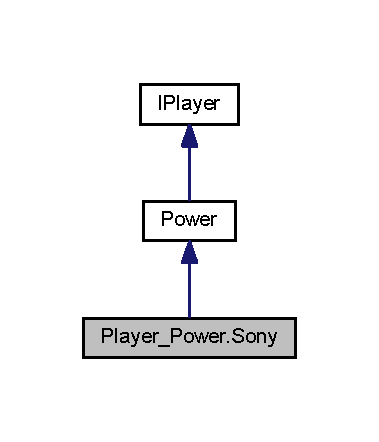
\includegraphics[width=182pt]{class_player___power_1_1_sony__inherit__graph}
\end{center}
\end{figure}


Граф связей класса Player\-\_\-\-Power.\-Sony\-:
\nopagebreak
\begin{figure}[H]
\begin{center}
\leavevmode
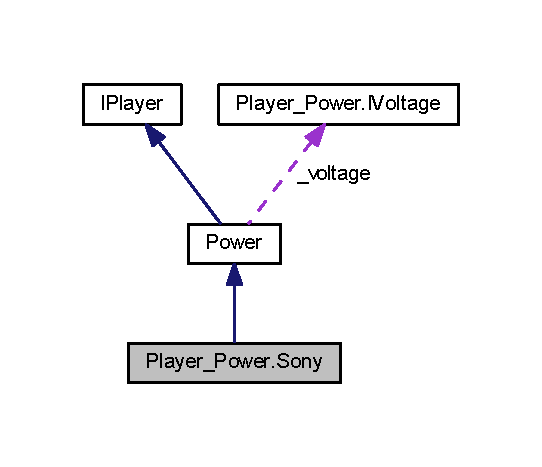
\includegraphics[width=260pt]{class_player___power_1_1_sony__coll__graph}
\end{center}
\end{figure}
\subsection*{Открытые члены}
\begin{DoxyCompactItemize}
\item 
{\bf Sony}({\bf I\-Player} player, {\bf I\-Voltage} \\*
voltage) override void {\bfseries Pause} ()\label{class_player___power_1_1_sony_a0a5ccde69df5a76581b50aa998763a1d}

\item 
override void {\bfseries Start} ()\label{class_player___power_1_1_sony_aecac16b26e060cc06f333ec92f9b58c4}

\item 
override void {\bfseries Stop} ()\label{class_player___power_1_1_sony_ab60d2550b44812f29357e1e5917c836e}

\item 
override void {\bfseries Show\-Voltage} ()\label{class_player___power_1_1_sony_a11c31dd40894bbccb3672084529359be}

\end{DoxyCompactItemize}
\subsection*{Дополнительные унаследованные члены}


Объявления и описания членов класса находятся в файле\-:\begin{DoxyCompactItemize}
\item 
Program.\-cs\end{DoxyCompactItemize}

%--- End generated contents ---

% Index
\newpage
\phantomsection
\addcontentsline{toc}{chapter}{Алфавитный указатель}
\printindex

\end{document}
